% !TeX program = xelatex 
\documentclass{hitreport}
\usepackage{url}
\usepackage{algorithm,float}  
\usepackage{algpseudocode}  
\usepackage{amsmath}
\usepackage{cite}
\usepackage{threeparttable}
\usepackage{subfig}
\usepackage{listings} %插入代码
\usepackage{xcolor} %代码高亮
\usepackage{tikz}
\usepackage{hyperref}
\usepackage{wasysym}
\usepackage{pgfplots}
\usetikzlibrary{positioning}




\lstset{numbers=left, %设置行号位置
	numberstyle=\tiny, %设置行号大小
	keywordstyle=\color{blue}, %设置关键字颜色
	commentstyle=\color[cmyk]{1,0,1,0}, %设置注释颜色
	frame=single, %设置边框格式
	escapeinside=``, %逃逸字符(1左面的键),用于显示中文
	breaklines, %自动折行
	extendedchars=false, %解决代码跨页时,章节标题,页眉等汉字不显示的问题
	xleftmargin=2em,xrightmargin=2em, aboveskip=1em, %设置边距
	tabsize=4, %设置tab空格数
	showspaces=false %不显示空格
}

\renewcommand{\algorithmicrequire}{\textbf{Input:}}  % Use Input in the format of Algorithm  
\renewcommand{\algorithmicensure}{\textbf{Output:}} % Use Output in the format of Algorithm  

\makeatletter
\newenvironment{breakablealgorithm}
  {% \begin{breakablealgorithm}
   \begin{center}
     \refstepcounter{algorithm}% New algorithm
     \hrule height.8pt depth0pt \kern2pt% \@fs@pre for \@fs@ruled
     \renewcommand{\caption}[2][\relax]{% Make a new \caption
       {\raggedright\textbf{\ALG@name~\thealgorithm} ##2\par}%
       \ifx\relax##1\relax % #1 is \relax
         \addcontentsline{loa}{algorithm}{\protect\numberline{\thealgorithm}##2}%
       \else % #1 is not \relax
         \addcontentsline{loa}{algorithm}{\protect\numberline{\thealgorithm}##1}%
       \fi
       \kern2pt\hrule\kern2pt
     }
  }{% \end{breakablealgorithm}
     \kern2pt\hrule\relax% \@fs@post for \@fs@ruled
   \end{center}
  }
\makeatother

% =============================================
% Part 0 Edit the info
% =============================================

\major{计算机科学与技术}
\name{孙骁}
\title{视听觉信号处理\\实验报告}
\stuid{1180300811} % 学号
\college{计算学部}
\date{2020年12月30日}
\lab{格物207} %实验地点
\course{视听觉信号处理}
\instructor{郑铁然}
% \grades{}
\expname{命令词(孤立词)识别实验} %实验名称
% \exptype{} % 实验类型
% \partner{} % 同组学生名字
\term{2020秋季学期}

\begin{document}

\maketitle

\tableofcontents
\newpage
% =============================================
% Part 1 Header
% =============================================



% =============================================
% Part 2 Main document
% =============================================

\section{实验目的和内容}

\subsection{实验目的}
\begin{enumerate}
\item 对语音识别技术进行动手实践;
\item 掌握基于DTW和基于HMM的命令词识别技术;
\item 设计一个命令词识别任务,定制词表,采集语料;
\item 能够设计和编写命令词识别的算法。
\end{enumerate}

\subsection{实验内容}
\begin{enumerate}

\item 设计命令词识别任务 

\begin{enumerate}
\item 设想一个任务,如智能家居、或车辆控制等;
\item 确定词表,要求词表中不少于5个词;
\item 录制语料。(Wav,16kHz,16bit). 每个词每人不少于10遍。对DTW算法,取其中一个实例为模板(每人一个),其它用于测试。对HMM算法,取其中7例(每人)为训练语料,3例(每人)为测试语料。可以用采集工具(如cooledit)或编程实现语音采集;
\item 检查语料。通过听辩检查来保证语料质量;
\item 去除静音。可以用端点检测算法实现,也可以手工实现。
\end{enumerate}

\item 特征提取
\begin{enumerate}
\item 每帧提取39维MFCC特征,帧长25ms,帧移10ms;
\item 可以采用HTK工具包中的hcopy命令实现(要求语料是WAV格式)
\item 显示内容
\end{enumerate}

\item DTW识别测试 

\begin{enumerate}
\item N个模板,M个待测命令词语料,进行N*M次DTW计算,得到N*M个DTW距离;
\item 每个DTW计算分成两步;

\begin{enumerate}
\item 分别载入模板和待测语料的MFCC特征矢量序列;
\item 计算两个特征序列的DTW距离。
\end{enumerate}

\end{enumerate}

\item 计算测试结果 

\begin{enumerate}
\item 每个测试语料都有一个类别标签$l_i$;
\item 每个测试语料都有一个识别结果$r_i$;

\begin{align}
r_i = \underset{j}{\arg \max}D_{ij}
\end{align}
其中,$D_{ij}$为第\textit{i}个测试语料和第\textit{j}个模板间的DTW距离(规整后)
\item 若$r_i = l_i$表示识别结果正确;
\item 计算正确率=识别结果正确的语料数/总测试语料数。

\end{enumerate}

\end{enumerate}

\section{实验环境}

\begin{enumerate}
\item Anaconda 4.8.4
\item Python 3.7.4
\item PyCharm 2020.3 (Professional Edition)
\item Windows 10 2004
\end{enumerate}

\section{实验原理}

\subsection{动态时间归正算法}\label{sec:energy}


动态时间弯折采用动态规划技术,将一个复杂的全局问题转化为许多局部最优问题,一步一步地进行决策。\cite{韩纪庆2019}假设参考模板的特征矢量序列为$\boldsymbol{X} = \left\{\boldsymbol{x}_1, \boldsymbol{x}_2, \cdots, \boldsymbol{x}_I\right\}$,输入语音特征矢量序列为$\boldsymbol{Y} = \left\{\boldsymbol{y}_1, \boldsymbol{y}_2, \cdots, \boldsymbol{y}_J\right\}$,$I\ne J$。DTW算法是寻找一个最佳的时间归正函数,使待测语音的时间轴\textit{j}非线性地映射到参考模板的时间轴\textit{i}上,使总累计失真率最小。

设时间归正函数为
\begin{align}
C=\left\{c\left(1\right), c\left(2\right), \cdots, c\left(N\right)\right\}
\end{align}
式中,\textit{N}为路径长度,$c\left(n\right)=\left(i\left(n\right),j\left(n\right)\right)$表示第\textit{n}个匹配点对是由参考模板的第$i\left(n\right)$个特征矢量与待测模板的第$j\left(n\right)$个特征矢量构成的匹配点对。两者之间的距离$d\left(\boldsymbol{x}_{i\left(n\right)}, \boldsymbol{y}_{j\left(n\right)}\right)$称为局部匹配距离。DTW算法就是通过局部优化的方法实现加权距离综合最小,即
\begin{align}
D = \underset{c}{\min} \frac{\sum\limits_{n=1}^{N}\left[d\left(\boldsymbol{x}_{i\left(n\right)}, \boldsymbol{y}_{j\left(n\right)}\right) \cdot W_n\right]}{\sum\limits_{n=1}^{N}}
\end{align}
式中,加权函数$W_n$对第\textit{n}对匹配点前一步局部路径的走向进行惩罚,对$45°$方向乘上乘法系数2,对于其他方向加上乘法系数1。

于是得到最小累计失真函数$g\left(i,j\right)$,表示到匹配点对$\left(i,j\right)$为止的前面所有可能的路径中最佳路径的累计匹配距离。$g\left(i,j\right)$存在如下递推关系:
\begin{align}
g\left(i,j\right) = \underset{\left(i',j'\right)\rightarrow\left(i,j\right)}{\min}\left\{g\left(i',j'\right)+d\left(x_i,y_i\right)W_n\right\}
\end{align}
其中,$\left(i',j'\right)$表示局部路径$\left(i',j'\right)\rightarrow \left(i,j\right)$的起点,权$W_n$的取值是与局部路径有关的。

则DTW算法递推求累计距离的核心公式为
\begin{align}
\begin{split}
g\left(i,j\right) = \min\{&g\left(i-1,j\right)+d\left(\boldsymbol{x}_i,\boldsymbol{y}_j\right)\times W_n\left(1\right),\\
&g\left(i-1,j-1\right)+d\left(\boldsymbol{x}_i,\boldsymbol{y}_j\right)\times W_n\left(2\right),\\
&g\left(i,j-1\right)+d\left(\boldsymbol{x}_i,\boldsymbol{y}_j\right)\times W_n\left(1\right)\}
\end{split}
\end{align}
其中,$i=2,3,\cdots,I;j=2,3,\cdots,J$,一般取距离权值$W_n\left(1\right) = 1$,$W_n\left(2\right) = 2$,于是得到了DTW算法。


\section{实验步骤及相应结果}

此部分内容与word模板相应章节对应,单击图片引用序号可以跳转查看相应图片结果。

\subsection{设计命令词识别任务}

\subsubsection{描述所设计的命令词识别任务}

收集5重不同饮品的名称,每种类别采集10遍语料,然后进行识别,程序判断新语料中饮品的类型后,指出种类。

\subsubsection{列出词表}

\begin{enumerate}
\item 茶
\item 咖啡
\item 果汁
\item 啤酒
\item 水
\end{enumerate}

\subsubsection{介绍语料采集方法和规模}

语料采集:Cool Edit,新建wav文件后,点击录音即可录制。第一次录制时杂音过多,调低电脑麦克风音量即可解决。
规模:一共五个关键词,每个关键词采集 10 次。

\subsection{特征提取}\label{sec:sec2}

\subsubsection{给出特征提取部分运行结果的截图}

特征提取的scp文件采用程序写入,由于自己的实验目录存在中文,hcopy无法使用utf8编码识别命令行中的中文,故将待提取特征的wav文件与提取结果放在D盘根目录下,写入scp文件的代码如下

\lstinputlisting[language=python]{code/write_list_scp.py}

在windows terminal中输入提取的命令:
\begin{lstlisting}[language=bash]
hcopy -A -D -T 1 -C tr_wav.cfg -S list1.scp
\end{lstlisting}

提取运行的结果如图(\ref{fig:feature})所示

\begin{figure}[htb]
	\centering
	\subfloat[特征提取第一段截图]{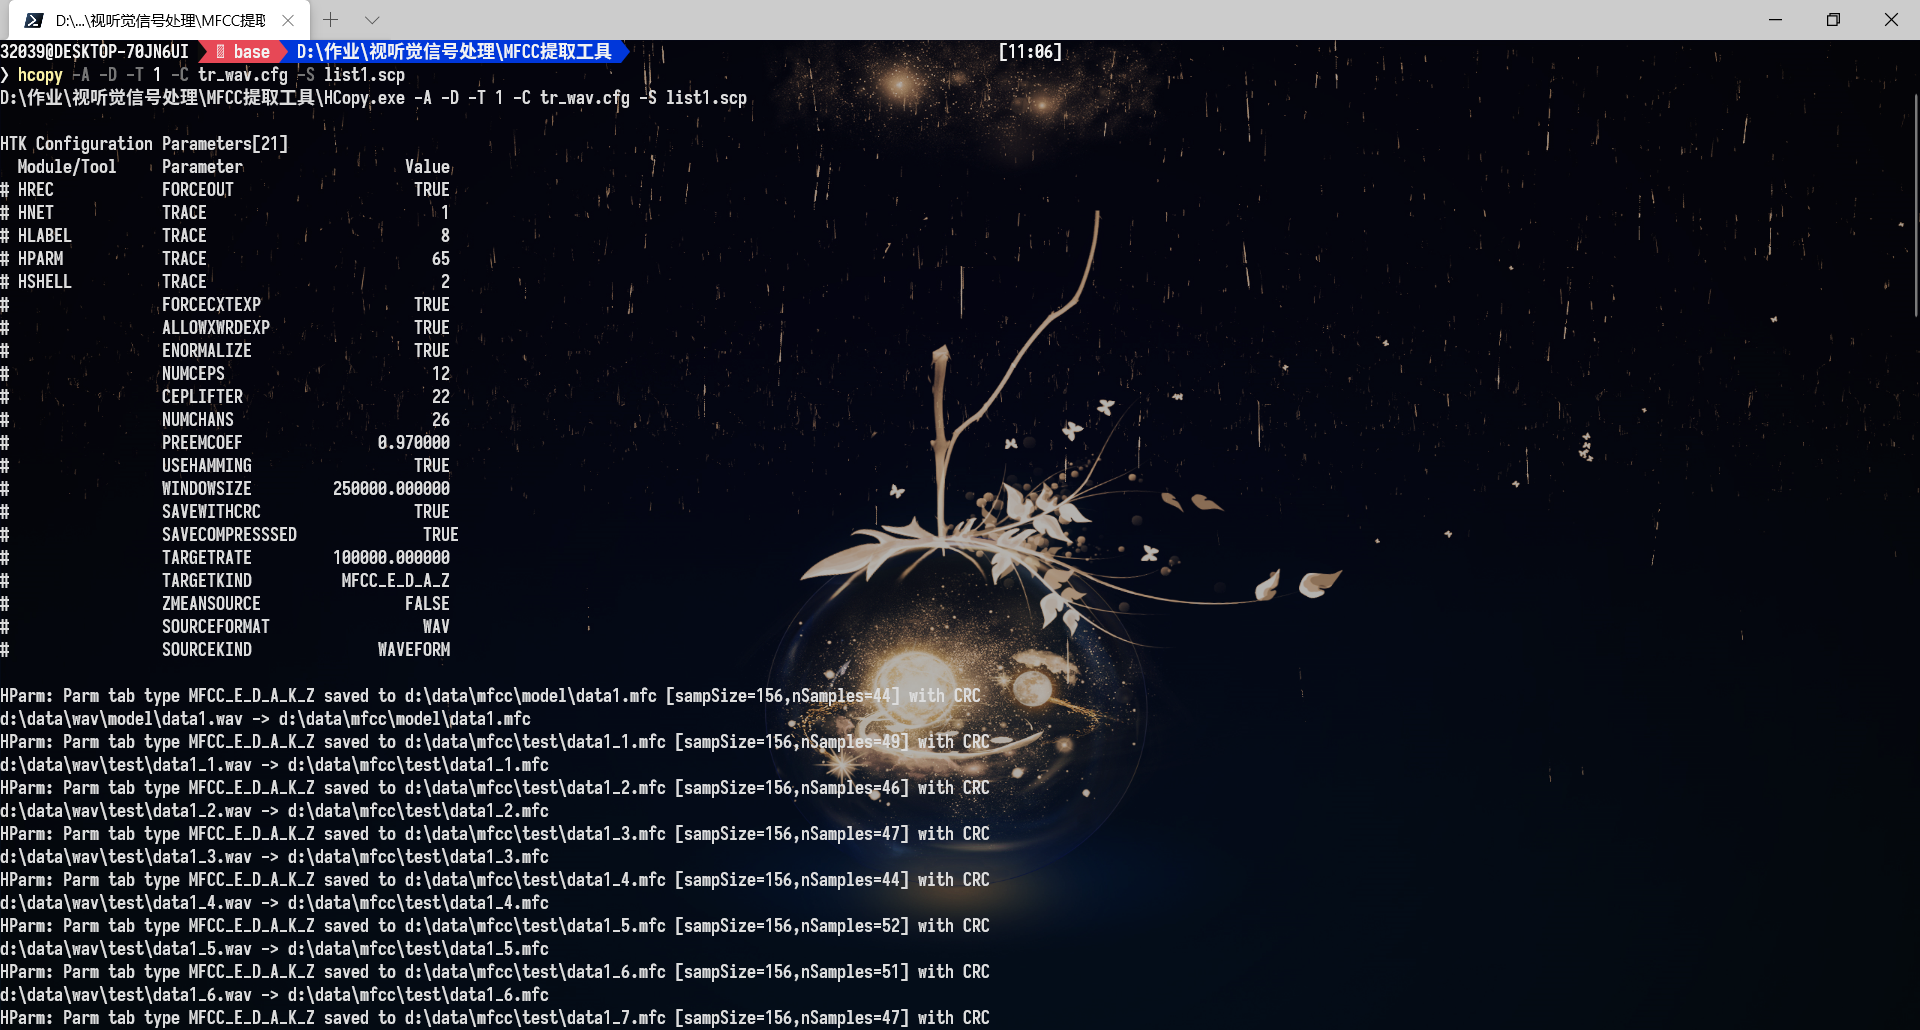
\includegraphics[width=0.6\linewidth]{fea1.png}}
	\\
	\subfloat[特征提取第二段截图]{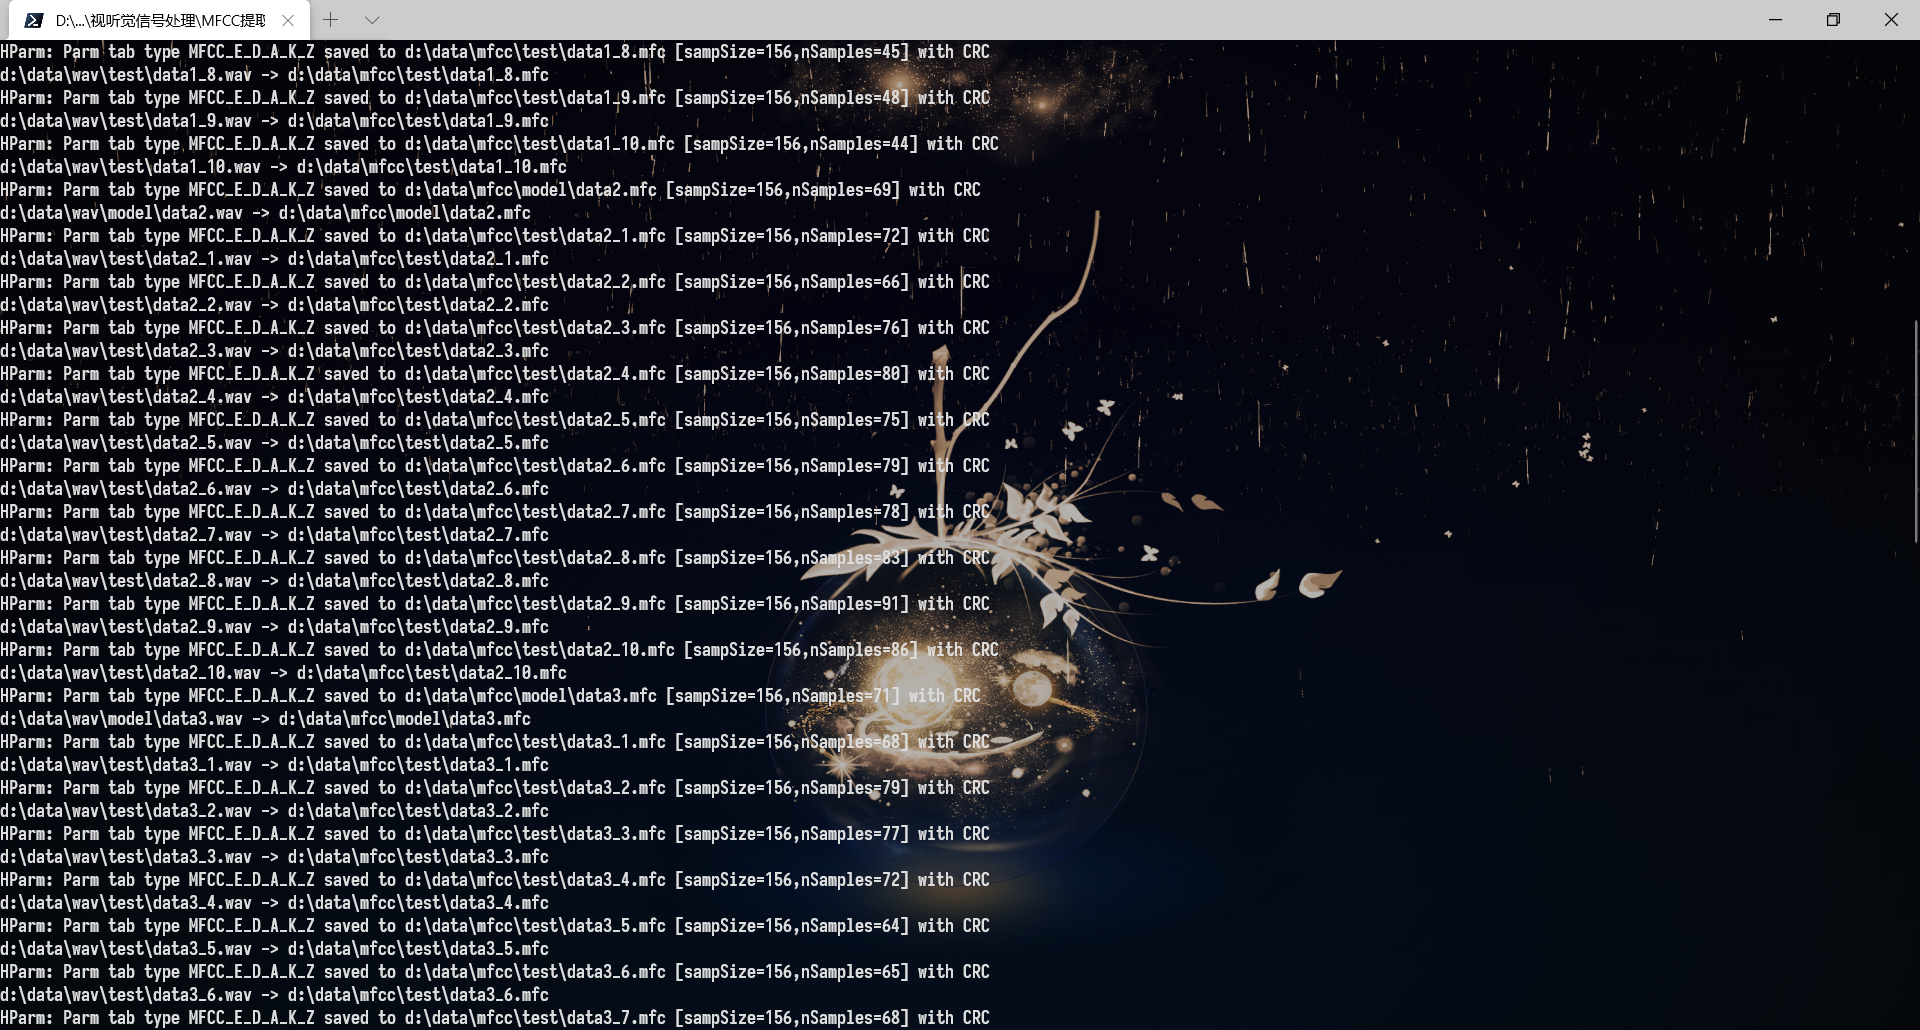
\includegraphics[width=0.6\linewidth]{fea2.png}}
	\\
	\subfloat[特征提取第三段截图]{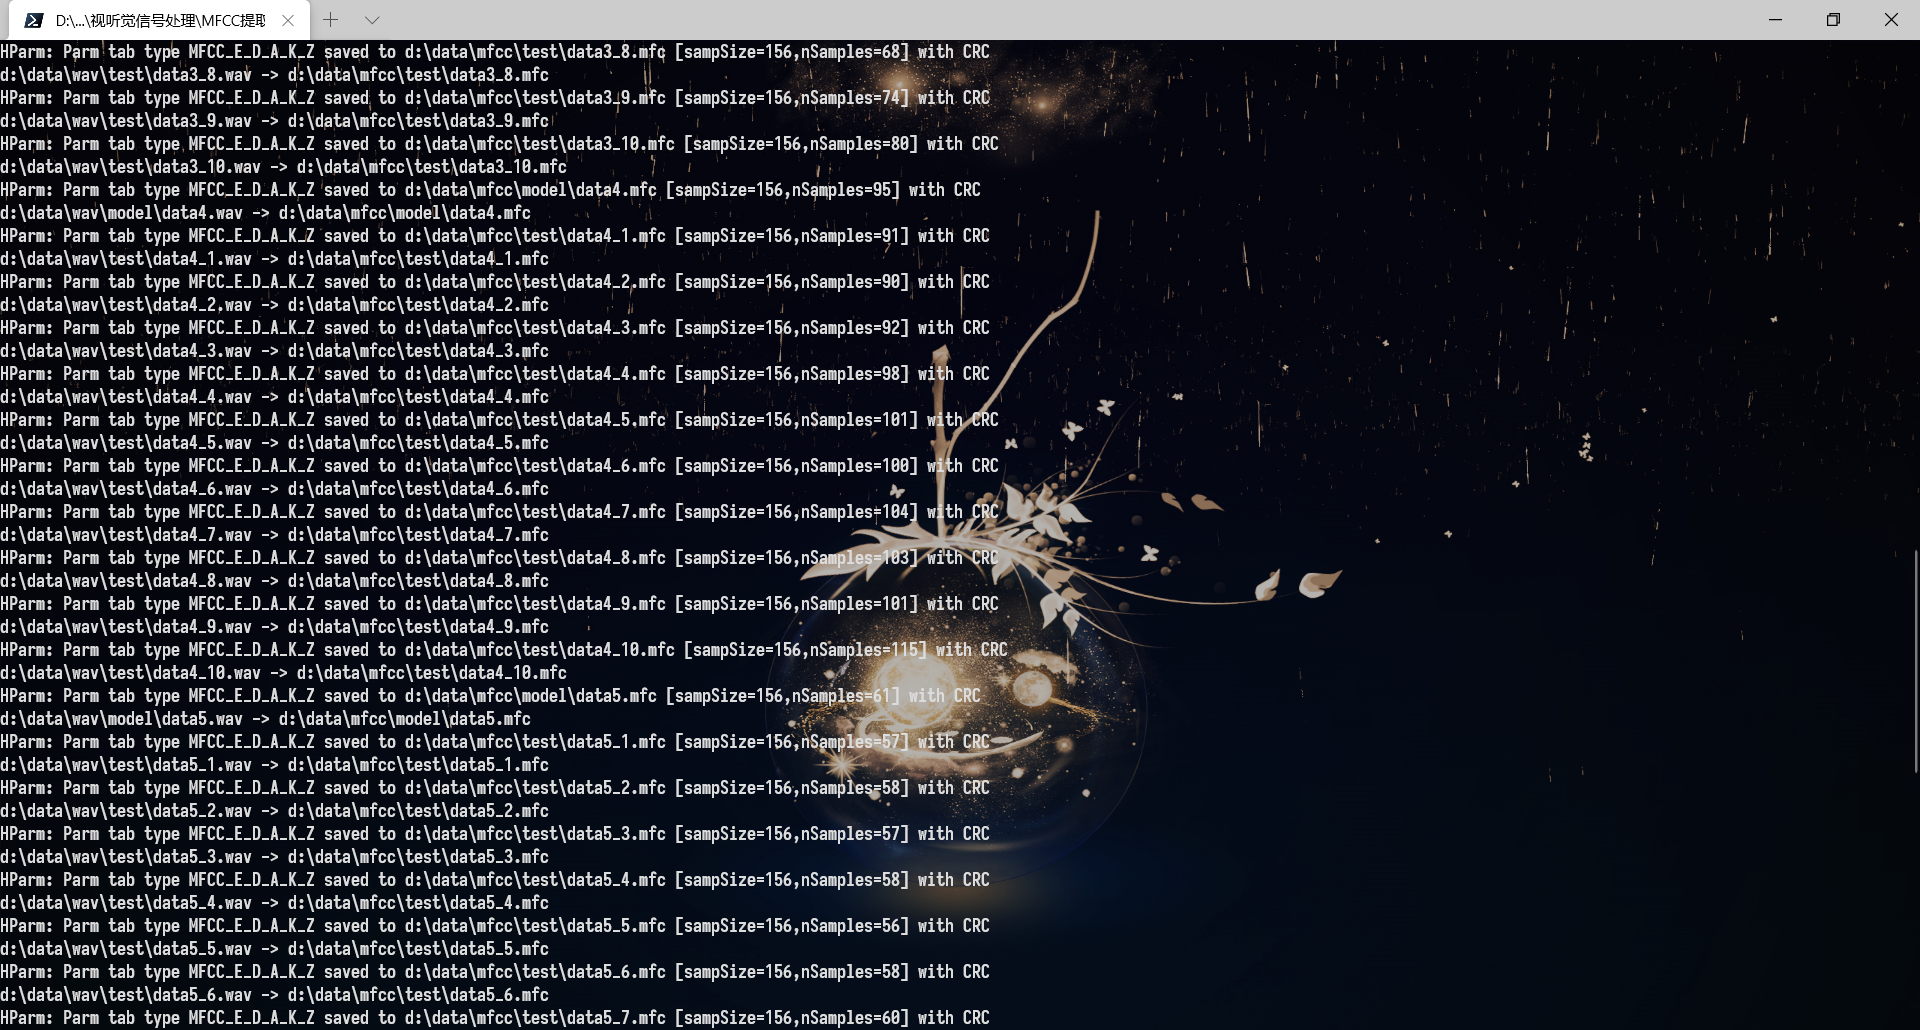
\includegraphics[width=0.6\linewidth]{fea3.png}}
	\\
	\subfloat[特征提取第四段截图]{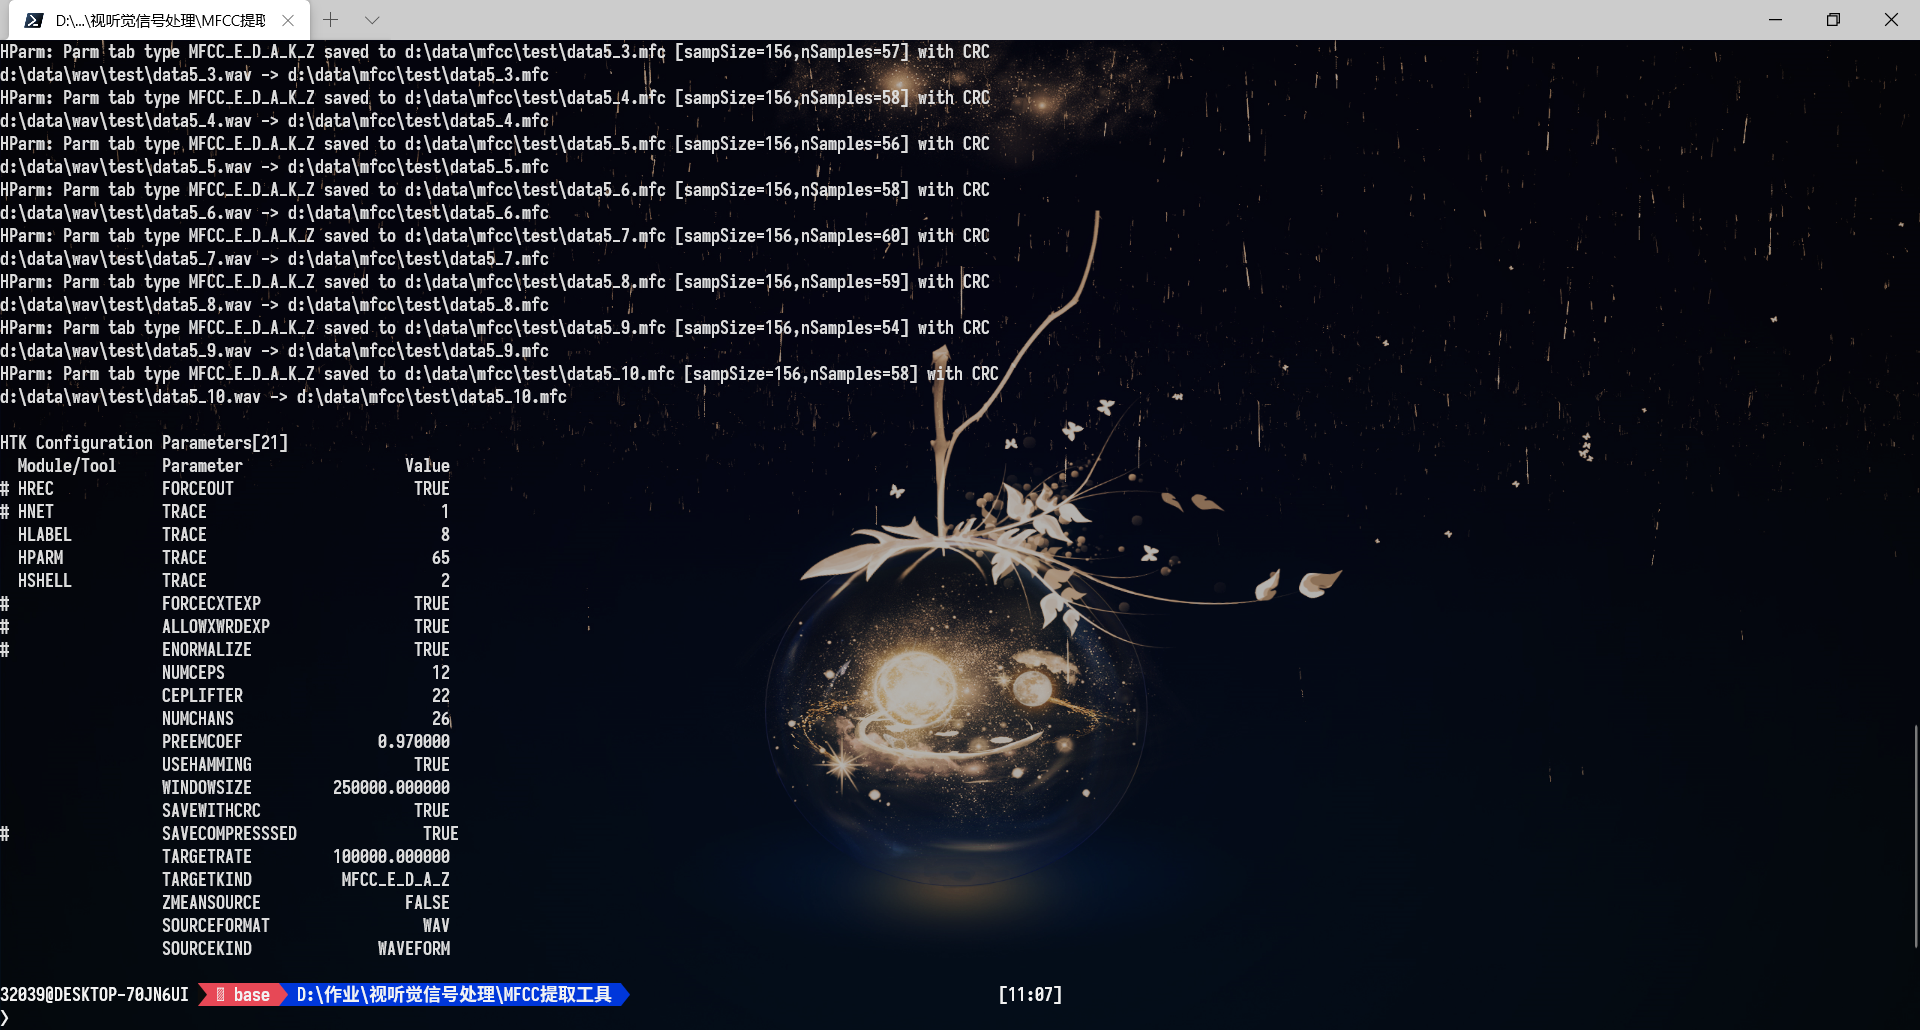
\includegraphics[width=0.6\linewidth]{fea4.png}}
	\caption{特征提取部分运行结果}\label{fig:feature}
\end{figure}

\subsection{基于DTW的命令词识别}\label{sec:sec4}

\subsubsection{介绍你所设计DTW算法,标明所采用的开发工具}

\paragraph{开发工具} Pycharm 2020.3
\paragraph{度量方式} 欧式距离

整体的核心代码如下:
\lstinputlisting[language=python]{code/dynamic_tme_warping.py}

\paragraph{算法描述}首先初始化最小累计失真函数cost\_matrix的各个位置为 0,然后初始化 cost\_matrix[0,:]和 cost\_matrix[:,0]
接下来进行动态规划,分别比较 cost\_matrix[i-1][j] + dis[i][j], cost\_matrix[i][j-1] + dis[i][j] 和
cost\_matrix[i-1][j-1] + dis[i][j]*2 的大小,取最小的一个,然后依次向下直到cost\_matrix[len\_vector1 - 1][len\_vector2 - 1]。

依次返回不同模板语料矢量动态规划的结果,选择类别为最小累计失真代价最小的模板,得到最终的识别正确率。

\subsubsection{正确率}

由于模板是5个,每个语料有10十个,控制台输出展示不下,因此将控制台输出重定向至log文件,得到的输出在log文件夹下可见,相应的时间为程序运行时间。实验写完较早,但是实验报告写完较晚。

识别正确率如最后一个log文件所示。五个语料的识别准确率均为100\%。
\lstinputlisting{code/2021-01-10-11-31.log}

\section{实验结论}

\begin{enumerate}
\item 使用DTW算法可以有效的解决特定说话人小规模的语音识别任务
\item 较大规模的语音识别任务应该使用基于HMM模型的语音识别算法
\end{enumerate}

 
\renewcommand\refname{参考文献}
 
\bibliographystyle{unsrt} %%参考文献的格式(可选的格式还有:plain)
 
\bibliography{Refer.bib}    %%参考文件存储位置

\newpage
\begin{appendices}

\section{DTW算法——dynamic\_tme\_warping.py}

\lstinputlisting[language=python]{code/dynamic_tme_warping.py}

\section{将控制台输出重定向至log文件——logger.py}

\lstinputlisting[language=python]{code/logger.py}

\section{主函数,程序入口——main.py}

\lstinputlisting[language=python]{code/main.py}

\section{从文件中读取已提取的mfcc特征——read\_mfcc\_from\_file.py}

\lstinputlisting[language=python]{code/read_mfcc_from_file.py}

\section{将待提取特征文件与提取就结果写入scp文件——write\_list\_scp.py}

\lstinputlisting[language=python]{code/write_list_scp.py}

\end{appendices}

\end{document}
